\chapter{Methodology}
Our method can be seen as an approach built upon the idea of leaf-root path or sub-path (section~\ref{leafrootmethod}), in an operation tree~\cite{goodsurvey}. 
But we have developed this idea further in many ways. 
Our index is composed from leaf-root paths from mathematical formulae operation tree. 
The search method is traversing a ``reversed" sub-path tree, coming along with a pruning method and a proposed sub-structure test algorithm, which are utilizing some observed properties from our indexed tree. 
Apart from these, we also offer several rules of constrains to measure symbolic similarity.
This chapter gives a summary on the method intuition and the core ideas behind these.

The methods in a nutshell is, for a document expression, construct operation tree and break it down into sub-paths, index those paths by inserting them into a tree-structured index by their reversed order. For a search query, traversal index tree as the same way of going through the reversed sub-paths of that query (search path), get the search results along the merged ways from different search paths. Finally apply symbol similarity measurement algorithm or the sub-structure test algorithm to rank results.

\section{Intuitions}
First it is beneficial to document our intuitions on using operation tree as our intermediate representation and our idea to index it in a way of “reversed” sub-path tree, and also explain in abstract why this way helps reduce index space and boost search speed.
We will give an illustrative example to describe these processes further in section~\ref{secIllu}.

\subsection{Commutative immunity}
Operators with semantic implication of commutative property (e.g. addition and multiplication) are exhaustively used in mathematical language. The ability to identify the identical equations for any permutation is very essential for a mathematical similarity search engine. 
Given this as a start point, the leaf-root paths have the advantage to cope this so that we do not need to generate different order of patterns to match formulae with commutative operator. 
To illustrate this, we know that a leaf-root path from an operation tree (see figure~\ref{oprtreeExample}) is generated through traversing in a bottom-up (or top-down) fashion from a tree, thus path string is independent with the relative position of operands from same father node.
In another word, an operation tree uniquely determines the leaf-node paths decomposed from the tree, no matter how operands are ordered. 

\subsection{Sub-structure query ability}
On the other hand, the structure of operation tree also makes it easy to represent sub-expression relation with a formula, because a sub-expression in a formula is usually (depending on the way we construct an operation tree) also a subtree in an operation tree. 
And by going up from leaves of operation tree, we are essentially traversing to an expression from its subexpression for every level. 
By making all the leaf-root paths as an index, we can search an expression by going through and beyond the leaf-root paths from its subexpression. 
This makes operation tree better in terms of searching an expression given a sub-expression in query. 
And it avoids information augmentation on index as some other structure-based methods need to do (e.g. index all sub-terms of an expression in MWS~\cite{Kohlhase06}). Therefore it helps save storage space. 

\subsection{Index and search properties}
Additionally, some properties from the ``inverted" of sub-paths (we will illustrate this in section~\ref{secIllu}) from an operation tree suggest some reduce of space and pruning possibilities in search process. 
First the sub-paths themselves can be indexed into a tree so that we can search a sub-path by traversing a sub-path tree, instead of hashing it to find a corresponding value as the symbol-pair search engine (i.e. \textit{Tangent}~\cite{symbolpairs15}) does. 
This allows us to save a lot space as the reverted sub-paths of a large collection will have a great percentage of level sharing a common string with each other. 
Also the way to search in a tree structure with a limited branch factor does not lose much efficiency compared to the HASH methods used in \textit{Tangent}, while also offer great storage efficiency.
Second, by searching from all the ``reverted" sub-paths of a query expression in our proposed index, and apply an intersection on the results from different sub-paths, we will find all the expressions have that query as subexpression (number four observed property from section~\ref{observationlabel}). And during this search process, upon going further from the query expression root in the ``reverted" sub-path, we can merge the next search directories by pruning all the entries that are not shared in common among all the ``reverted" search path directories. 
Further more, multiple index search in different path level are independent with each other, put in another way, if a given indexed formula has been found in one search path level, then its other relevant sub-paths (in terms of the current query) will most likely be found at the same search level too, thus some implementation strategies can be applied to speed search further (i.e. distributed search to quick search massive), which we would address in the next chapter.

\begin{figure}
\begin{minipage}[b]{2.65in}
\begin{center}
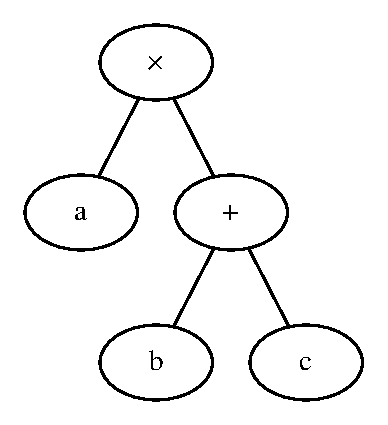
\includegraphics[height=1.8in]{leafroottree}
\\$a(b+c)$ in operation tree
\end{center}
\end{minipage}
\hspace*{.38in}
\begin{minipage}[b]{2.65in}
\begin{center}
\raisebox{.0in}{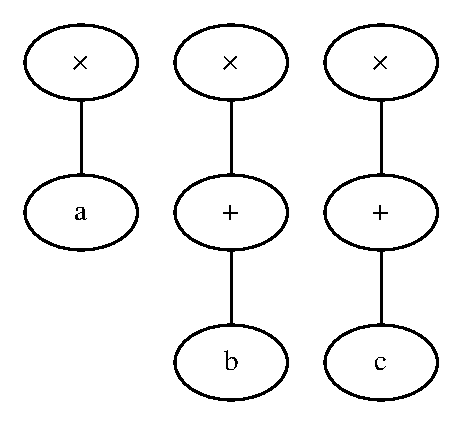
\includegraphics[height=1.8in]{leafrootpath}}
Generated leaf-root paths
\end{center}
\end{minipage}
\caption{Leaf-Root Path Example}\label{oprtreeExample}
\end{figure}

\section{Structure Similarity}
The basic ideas used in our approach, to test whether a mathematical expression is an sub-structure of another, to prune and to constrain search process are the foundation work in our research. It is desired to give a description in a formal language so that we can deliver these ideas in the most precise way. Some important observations as well as brief justifications are provided after definitions.

\subsection{Definitions}
For the second issue addressed in section~\ref{measure_sim}, specifically, to assess the structural similarity. 
Previous formal definitions~\cite{improving09} have been given on this, providing a quantified \mbox{$n$-similarity} relation to address the similarity degree, which is determined by the max-weight common subtree between two formulae. 
The subtree, by their definition, includes all descendants from a node. 
Nevertheless, we are going to use the subtree definition in graph theory here to describe the sub-structure relation. 
To be explicit, given a rooted tree $T$, the connected graph whose edges are also in $T$ is defined as the subtree of $T$.  

Based upon this,  we introduce a \textit{formula subtree} relation to address the sub-structure relation between two mathematical expressions. 
The formula tree is associated with a label (labels are not required to be distinct here) in each node to represent a mathematical operator, variable, constance etc., also a symbol value in each leaf node to represent a symbolic instance of that constance or variable (e.g. ``123", $\beta$, \textit{x, y} etc.). 
Below are our formal definitions.

\subsubsection{Formula tree}
Formula tree is a labeled rooted non-empty tree $T = T(V,E,r)$ with root $r$, where each vertices $v \in V(T)$ is associated with a label $\ell(v) \in \mathbf{R}$ mapped by function $\ell$, and each leaf $l \in V(T)$ is also associated with a symbol $s(v) \in \mathbf{R}$ mapped by function $s$.

\subsubsection{Formula subtree}
Given formula tree $S$ and $T$, we say $S$ is a formula subtree of $T$ if there exists an injective mapping $\phi: V(S) \rightarrow V(T)$ satisfying:

\begin{enumerate}
\item 
$\forall\; (v_1,v_2) \in E(S)$, we have $(\phi(v_1),\phi(v_2)) \in E(T)$;
\item
$\forall\; v \in V(S)$, we have $\ell(v) = \ell(\phi(v))$;
\item
If $v \in V(S)$ is a leaf vertices in $S$, then $\phi(v)$ is also a leaf in $T$.
\end{enumerate}
Such a mapping $\phi$ is called a formula subtree isomorphic embedding (or formula embedding) for $S \rightarrow T$. 
If satisfied, we denote $S \preceq_l T$ on $\Phi$, where $\Phi$ ($\Phi \neq \emptyset$) is the set of all the possible formula embeddings for $S \rightarrow T$.

\subsection{Observations}
\label{observationlabel}
\subsubsection*{Observation \#1} 
For two formula trees which satisfy $T_q \preceq_l T_d$ on $\Phi$, then $\forall\; \phi \in \Phi,\, p \in g(T_q)$, also any vertices $v$ along path $p$, the following properties are obtained:
\begin{eqnarray}
\deg(v) \le \deg(\phi(v)) \label{prop1} \\
\left| p \right| = \left| \phi(p) \right| \label{prop2} \\
\ell(p) = \ell(\phi(p)) \label{prop3} \\
\left| g(T_q) \right| \le \left| g(T_d) \right| \label{prop4}
\end{eqnarray}
\textit{Justification.} 
Because $\forall\; w \in V(T_q) \  s.t. \  (v, w) \in E(T_q)$, there exists $(\phi(v), \phi(w)) \in E(T_d)$. 
And for any (if exists) two different edges $(v, w_1), (v, w_2) \in E(T_q),\, w_1 \not= w_2 \in V(T_q) $, we know $(\phi(v), \phi(w_1)) \not= (\phi(v), \phi(w_2))$ by the formula subtree definition. 
Therefore any different edge from $v$ is associated with a distinct edge from $\phi(v)$, thus we can get \ref{prop1}. 
Given the fact that every non-empty path $p$ can be decomposed into a series of edges $(p_0, p_1), (p_1, p_2) \ldots (p_{n-1}, p_n), \; n > 0$,
properties \ref{prop2} and \ref{prop3} are trivial.
Because there is exact one path between every two nodes in a tree, the leaf-root path is uniquely determined by a leaf node in a tree. Hence the rationale of \ref{prop4} can be obtained in a similar manner with that of \ref{prop1}, expect neighbor edges are replaced by leaf-node paths.


\subsubsection*{Observation \#2} 
Given two formula trees $T_q$ and $T_d$, if $\left| g(T_q) \right| = 1$ and $\ell(g(T_{q})) \subseteq \ell(g(T_d))$, then $T_q \preceq_l T_d$.

\noindent \textit{Justification.} 
Obviously there is only single one leaf-root path in $T_q$ because $\left| g(T_q) \right| = 1$. 
Denote the path as $p = p_0 \ldots p_n,\; n \ge 0$ where $p_n$ is the leaf, and let $a = \ell(p)$.
Since $a \subseteq \ell(g(T_d))$, we know that there must exist a path $p'=p'_0 \ldots p'_n \in g(T_d)$ such that $a = \ell(p')$.
Without loss of generality, suppose $p'_n$ is the leaf of $T_d$. 
Now the injective function $\phi: p_i \rightarrow p'_i,\  0 \le i \le n$ satisfies all the requirements for $T_q$ as a formula subtree of $T_d$.

\subsubsection*{Observation \#3} 
For two formula trees $T_q$ and $T_d$, if $T_q = T(V,E,r) \preceq_l T_d$ on $\Phi$,  
$\forall a,b \in g(T_q)$ and a mapping $\phi \in \Phi$. 
Let $T_d' = \, ^{t}T_d$ where $t = \phi(r)$ and $a' = \phi(a)$, $\forall\; b' \in g(T_d')$, it follows that:
$$
\begin{array}{lcr}
b' = \phi(b)  & \Rightarrow & 
\left| \mathrm{lcp}(a,b) \right| = \left| \mathrm{lcp}(a',b') \right|
\end{array}
$$
Furthermore, $\forall\; c \in g(T_q)\; s.t.\; \left| \mathrm{lcp}(a,b) \right| \neq \left| \mathrm{lcp}(a,c) \right| $, we have
$$
\begin{array}{lcr}
\left| \mathrm{lcp}(a,b) \right| = \left| \mathrm{lcp}(a',b') \right|
& \Rightarrow &
b' \neq \phi(c)
\end{array} 
$$
\textit{Justification.} 
Because $a,b \in g(T_q)$, thus $a_0 = b_0 = r$, we make sure $\mathrm{lcp}(a,b) \ge 1$. 
Denote the path of $a = a_0 \ldots a_n a_{n+1} \ldots a_{l-1}$, similarly the path of $b=b_0 \ldots b_n b_{n+1} \ldots b_{m-1}$,
where the length of each $l,m \ge 1$ and $a_i = b_i,\, 0 \le i \le n \le \min(l-1, m-1)$ while $a_{n+1} \neq b_{n+1}$ if $l,m > 1$.
On the other hand $a' = \phi(a)$ and $b' \in g(\,^{t}T_d)$, therefore $a'_0 = \phi(a_0) = \phi(r) = t = b'_0$.
For the first conclusion, if $b' = \phi(b)$, there are two cases. If any of $|a|$ or $|b|$ is equal to one then $\left| \mathrm{lcp}(a,b) \right| = |(r)| = |(t)| = \left| \mathrm{lcp}(a',b') \right| = 1$;
Otherwise if $l,m > 1$, path $a_0 \ldots a_n = b_0 \ldots b_n$ and $a_{n+1} \neq b_{n+1}$ follow that $\phi(a_0 \ldots a_n) = \phi(b_0 \ldots b_n)$ and $\phi(a_{n+1}) \neq \phi(b_{n+1})$ by definition.
Because edge $(\phi(a_n), \phi(a_{n+1}))$ and $(\phi(b_n), \phi(b_{n+1}))$ are also in $E(T'_d)$, 
we see $\left| \mathrm{lcp}(a,b) \right| = \left| \mathrm{lcp}(a',b') \right| = n$.
For the second conclusion, we prove by contradiction. 
Assume $b' = \phi(c)$, by the first conclusion we know $\left| \mathrm{lcp}(a,c) \right| = \left| \mathrm{lcp}(a',b') \right|$.
On the other hand, because $\left| \mathrm{lcp}(a,c) \right| \neq \left| \mathrm{lcp}(a,b) \right| =  \left| \mathrm{lcp}(a',b') \right|$, 
thus $\left| \mathrm{lcp}(a,c) \right| \neq \left| \mathrm{lcp}(a',b') \right|$ which is impossible. 

\subsubsection*{Observation \#4} 
Given an index $\Pi$ and a formula tree $T_q$, $\forall\; T_d \in \Pi$:
If $T_q \preceq_l T_d$ on $\Phi$, then $\exists\; \hat{a} \in \mathbf{L},\; s.t.$
$$
T_d \in \bigcap_{a \in L} \mathcal{I}_{\Pi}(a)
$$
where $L = \ell(g(T_q)) \cdot \hat{a}$.

\noindent \textit{Justification.} 
Denote the root of $T_q$ and $T_d$ as $r$ and $s$ respectively. 
Let a path $\hat{p}$ be the path determined by 

\subsection{Interpretation}

\section{Symbolic Similarity}
Until now, we have not addressed symbolic similarity yet.
\subsection{Constrains and one step back}
\subsection{Mark-and-cross algorithm}
However, another shortcoming is, they usually fail to achieve the desired property for preserving same similarity when changes are made by substitution (see section~\ref{measure_sim}).

we doubt that users are likely to query, for example a+b c want-
ing to find documents only with occurrences of variable c.

Further more, a query may be specified with wildcards and thus will match any document with an expression substitution to that wildcard. 

The definition of similarity between two mathematical expressions is a key con-
cept that significantly affects a mathematical information retrieval system, but
a formal definition of similarity is missing in the literature. Here we formally
define the similarity between two mathematical expressions

\section{Illustrated by An Example}
\label{secIllu}

\section{Review on the Method}

Analogously,
Breakdown

Our system Cowpie \footnote{demo page: \url{infolab.ece.udel.edu:8912/cowpie/}}

\let\thefootnote\relax\footnote{Contact author: clock126@126.com or
\url{http://www.eecis.udel.edu/~zhongwei}}

MathML vs LaTeX
